\documentclass{article}

\usepackage{amsmath,amssymb,amsthm}
\usepackage{listings}
\usepackage{graphicx}
\usepackage[shortlabels]{enumitem}
\usepackage{tikz}
\usepackage[margin=1in]{geometry}
\usepackage{fancyhdr}
\usepackage{epsfig} %% for loading postscript figures
\usepackage{amsmath}
\usepackage{float}
\usepackage{amssymb}
\usepackage{caption}
\usepackage{subfigure}
\usepackage{graphics}
\usepackage{titlesec}
\usepackage{mathrsfs}
\usepackage{amsfonts}
\usepackage{indentfirst}
\usepackage{color}
\usepackage{algorithm}
\usepackage{algorithmicx}
\usepackage{algpseudocode}
\renewcommand{\baselinestretch}{1.2}%Adjust Line Spacing
%\geometry{left=2.0cm,right=2.0cm,top=2.0cm,bottom=2.0cm}% Adjust Margins of the File
\usepackage{tikz-qtree}
\usetikzlibrary{graphs}
\tikzset{every tree node/.style={minimum width=2em,draw,circle},
	blank/.style={draw=none},
	edge from parent/.style=
	{draw,edge from parent path={(\tikzparentnode) -- (\tikzchildnode)}},
	level distance=1.2cm}
\setlength{\parindent}{0pt}
%\setlength{\parskip}{5pt plus 1pt}
\setlength{\headheight}{13.6pt}
\newcommand\question[2]{\vspace{.25in}\hrule\textbf{#1: #2}\vspace{.5em}\hrule\vspace{.10in}}
\renewcommand\part[1]{\vspace{.10in}\textbf{(#1)}}
%\newcommand\algorithm{\vspace{.10in}\textbf{Algorithm: }}
\newcommand\correctness{\vspace{.10in}\textbf{Correctness: }}
\newcommand\runtime{\vspace{.10in}\textbf{Running time: }}
\pagestyle{fancyplain}
% Create horizontal rule command with an argument of height
\newcommand{\horrule}[1]{\rule{\linewidth}{#1}}



% Set the title here
\title{
	\normalfont \normalsize
	\textsc{ShanghaiTech University} \\ [25pt]
	\horrule{0.5pt} \\[0.4cm] % Thin top horizontal rule
	\huge CS101 Algorithms and Data Structures\\ % The assignment title
	\LARGE Fall 2021\\
	\LARGE Homework 4\\
	\horrule{2pt} \\[0.5cm] % Thick bottom horizontal rule
}
% wrong usage of \author, never mind
\author{}
\date{Due date: 23:59, October 24, 2021}

% set the header and footer
\pagestyle{fancy}
\lhead{CS101 Algorithms and Data Structures}
\chead{Homework 4}
\rhead{Due date: 23:59, October 24, 2021}
\cfoot{\thepage}
\renewcommand{\headrulewidth}{0.4pt}
\newtheorem{Q}{Question}
% special settings for the first page
\fancypagestyle{firstpage}
{
	\renewcommand{\headrulewidth}{0pt}
	\fancyhf{}
	\fancyfoot[C]{\thepage}
}

% Add the support for auto numbering
% use \problem{title} or \problem[number]{title} to add a new problem
% also \subproblem is supported, just use it like \subsection
\newcounter{ProblemCounter}
\newcounter{oldvalue}
\newcommand{\problem}[2][-1]{
	\setcounter{oldvalue}{\value{secnumdepth}}
	\setcounter{secnumdepth}{0}
	\ifnum#1>-1
	\setcounter{ProblemCounter}{0}
	\else
	\stepcounter{ProblemCounter}
	\fi
	\section{Problem \arabic{ProblemCounter}: #2}
	\setcounter{secnumdepth}{\value{oldvalue}}
}
\newcommand{\subproblem}[1]{
	\setcounter{oldvalue}{\value{section}}
	\setcounter{section}{\value{ProblemCounter}}
	\subsection{#1}
	\setcounter{section}{\value{oldvalue}}
}

% \setmonofont{Consolas}
\definecolor{blve}{rgb}{0.3372549 , 0.61176471, 0.83921569}
\definecolor{gr33n}{rgb}{0.29019608, 0.7372549 , 0.64705882}
\makeatletter
\lst@InstallKeywords k{class}{classstyle}\slshape{classstyle}{}ld
\makeatother
\lstset{language=C++,
	basicstyle=\ttfamily,
	keywordstyle=\color{blve}\ttfamily,
	stringstyle=\color{red}\ttfamily,
	commentstyle=\color{magenta}\ttfamily,
	morecomment=[l][\color{magenta}]{\#},
	classstyle = \bfseries\color{gr33n}, 
	tabsize=4
}
\lstset{basicstyle=\ttfamily}
\begin{document}

\maketitle
\thispagestyle{firstpage}
%\newpage
\vspace{3ex}

\begin{enumerate}
	\item Please write your solutions in English.

	\item Submit your solutions to gradescope.com.

	\item Set your FULL NAME to your Chinese name and your STUDENT ID correctly in Account Settings.

	\item If you want to submit a handwritten version, scan it clearly. Camscanner is recommended.

	\item When submitting, match your solutions to the according problem numbers correctly.

	\item No late submission will be accepted.

	\item Violations to any of the above may result in zero grade.

	\item Problem 0 gives you a template on how to organize your answer, so please read it carefully.
\end{enumerate}
\newpage

\problem[0]{Notes and Example}
\textbf{Notes}
\begin{enumerate}
	\item Some problems in this homework requires you to design Divide and Conquer algorithm. When grading these problems, we will put more emphasis on how you reduce a problem to a smaller size problem and how to combine their solutions with Divide and Conquer strategy.
	\item Your answer for these problems should include:
	      \begin{enumerate}
		      \item Algorithm Design
		      \item Time Complexity Analysis
		      \item Pseudocode (Optional)
	      \end{enumerate}
	\item In Algorithm Design, you should describe each step of your algorithm clearly.
	\item Unless required, writing pseudocode is optional. If you write pseudocode, please give some additional descriptions if the pseudocode is not obvious.
	\item You are recommended to finish the algorithm design part of this homework with \LaTeX.
\end{enumerate}

\newpage
\noindent
\question{0}{Binary Search Example}

\textit{Given a sorted array $a$ of $n$ elements, design an algorithm to search for the index of given element $x$ in $a$.\\}

\vspace{1em}
\noindent
\textbf{Algorithm Design:}
We basically ignore half of the elements just after one comparison.\\
\begin{enumerate}
	\item Compare $x$ with the middle element.
	\item If $x$ matches with the middle element, return the middle index.
	\item Else If $x$ is greater than the mid element, then $x$ can only lie in right half subarray after the mid element. So we recur for right half.
	\item Otherwise ($x$ is smaller) recur for the left half.
\end{enumerate}

~\\

\textbf{Pseudocode(Optional):}\\
$left$ and $right$ are indecies of the leftmost and rightmost elements in given array $a$ respectively.
\begin{algorithm}[H]
	\begin{algorithmic}[1]
		\Function {binarySearch}{a, value, left, right}
		\If {right $<$ left}
		\State \Return not found
		\EndIf
		\State mid $\gets \lfloor (right-left)/2 \rfloor + left$
		\If {a[mid] = value}
		\State \Return mid
		\EndIf
		\If {value $<$ a[mid]}
		\State \Return binarySearch(a, value, left, mid-1)
		\Else
		\State \Return binarySearch(a, value, mid+1, right)
		\EndIf
		\EndFunction
	\end{algorithmic}
\end{algorithm}

~\\

\textbf{Time Complexity Analysis:}
During each recursion, the calculation of $mid$ and comparison can be done in constant time, which is $O(1)$. We ignore half of the elements after each comparison, thus we need $O(\log n)$ recursions.
$$T(n) = T(n/2)+O(1)$$\\
Therefore, by the Master Theorem $\log_{b}{a}=1=d$, so $T(n) = O(\log n)$.

\newpage



\question{1}{(2' + 2' + 2') Trees}
Each question has \textbf{exactly one} correct answer. Please answer the following questions \textbf{according to  the definition specified in the lecture slides}.\\

\textit{Note: Write down your answers in the table below. }
\begin{table}[htbp]
	\begin{tabular}{|p{2cm}|p{2cm}|p{2cm}|p{2cm}|p{2cm}|p{2cm}|}
		\hline
		Question 1 & Question 2 & Question 3 \\
		\hline
		D          & B          & A          \\
		\hline
	\end{tabular}
\end{table}

\begin{Q}
	Which of the following statements is true?
	\begin{enumerate}[(A)]
		\item Each node in a tree has exactly one parent pointing to it.
		\item Nodes with the same ancestor are siblings.
		\item The root node cannot be the descendant of any node.
		\item Nodes whose degree is zero are also called leaf nodes.
	\end{enumerate}
\end{Q}
\vspace{0.5cm}


\begin{Q} Given the following pseudo-code, what kind of traversal does it implement?

	\begin{algorithm}[H]
		\begin{algorithmic}[1]
			\Function {order}{node}
			\If{node has left child}
			\State order(node.left)
			\EndIf

			\If{node has right child}
			\State order(node.right)
			\EndIf

			\State visit(node)
			\EndFunction
		\end{algorithmic}
	\end{algorithm}


	\begin{enumerate}[(A)]
		\item Preorder depth-first traversal
		\item Postorder depth-first traversal
		\item Inorder depth-first traversal
		\item Breadth-first traversal
	\end{enumerate}
\end{Q}

\vspace{0.5cm}

\pagebreak

\begin{Q} Which traversal strategy should we use if we want to print the hierachical structure ?

	\begin{figure}[h]
		\centering
		\includegraphics[width=0.27\linewidth]{hierarchy}
		\label{fig:hierarchy}
	\end{figure}
	\begin{enumerate}[(A)]
		\item Preorder depth-first traversal
		\item Postorder depth-first traversal
		\item Inorder depth-first traversal
		\item Breadth-first traversal
	\end{enumerate}
\end{Q}


\question{2}{(3+3+3pts) Tree Structure and Traversal}

Answer the following questions for the tree shown below \textbf{according to  the definition specified in the lecture slides}.

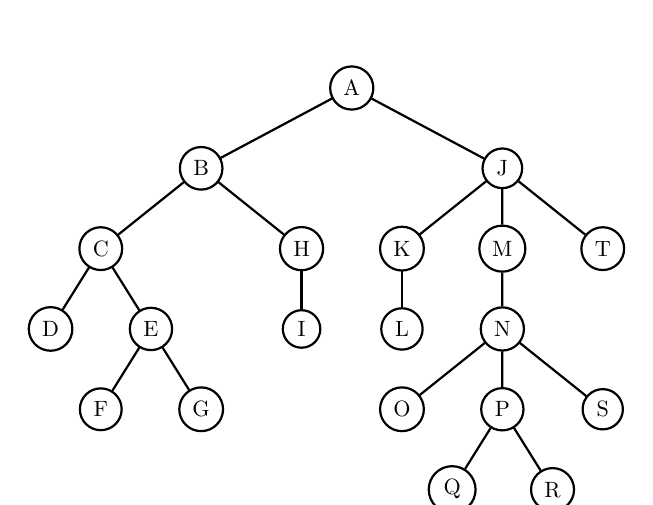
\begin{tikzpicture}
	[thick,scale=0.85, every node/.style={scale=0.8}]

	\node [circle,draw] {A}
	child {node [circle,draw] {B}
			child {node [circle,draw] {C}
					child {node [circle,draw] {D}}
					child {node [circle,draw] {E}
							child {node [circle,draw] {F}}
							child {node [circle,draw] {G}}
						}
				}
			child [missing] {}
			child {node [circle,draw] {H}
					child {node [circle,draw] {I}}
				}
		}
	child [missing] {}
	child [missing] {}
	child {node [circle,draw] {J}
			child {node [circle,draw] {K}
					child {node [circle,draw] {L}}
				}
			child {node [circle,draw] {M}
					child {node [circle,draw] {N}
							child {node [circle,draw] {O}}
							child {node [circle,draw] {P}
									child {node [circle,draw] {Q}}
									child {node [circle,draw] {R}}
								}
							child {node [circle,draw] {S}}
						}
				}
			child {node [circle,draw] {T}}
		};
\end{tikzpicture}
\begin{Q} Please specify:
	\begin{enumerate}[1.]
		\item The \textbf{children} of the \textbf{root node} with their \textbf{degree} respectively.	B(2),J(3)
		\item All \textbf{leaf nodes} in the tree with their \textbf{depth} respectively.	D(3),F(4),G(4),I(3),L(3),O(4),Q(5),R(5),S(4),T(2)
		\item The \textbf{height} of the tree.	height:5
		\item The \textbf{ancestors} of O.	O,N,M,J,A
		\item The \textbf{descendants} of C.	C,D,E,F,G
		\item The \textbf{path} from A to S.	(A,J,M,N,S)
	\end{enumerate}
\end{Q}

For the following two questions, traverse the \textbf{subtree} of the tree shown above with specified root.\\

Note: Form your answer in the following steps.
\begin{enumerate}[1.]
	\item Decide on an appropriate \textbf{data structure} to implement the traversal.
	\item When you are pushing the children of a node into a \textbf{queue}, please push them alphabetically i.e. from left to right; when you are pushing the children of a node into a \textbf{stack}, please push them in a reverse order i.e. from right to left.
	\item \textbf{Show all current elements in your data structure at each step} clearly  . \textbf{Popping a node} or \textbf{pushing a sequence of children} can be considered as one single step.
	\item \textbf{Write down your traversal sequence} i.e. the order that you pop elements out of the data structure.
\end{enumerate}

Please refer to the examples displayed in the lecture slide for detailed implementation of traversal in a tree using the data structure.


\vspace{0.1cm}
\begin{Q}
	Run \textbf{Depth First Traversal} in the subtree with root B.
\end{Q}

\vspace{0.5cm}
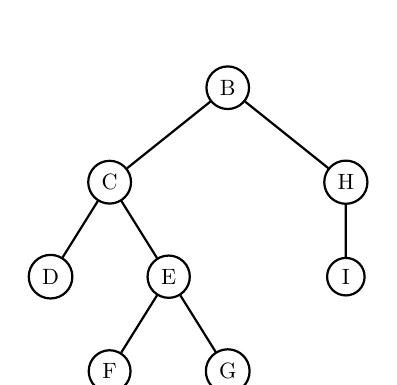
\begin{tikzpicture}
	[thick,scale=1.0, every node/.style={scale=0.8}]
	\node [circle,draw] {B}
	child {node [circle,draw] {C}
			child {node [circle,draw] {D}}
			child {node [circle,draw] {E}
					child {node [circle,draw] {F}}
					child {node [circle,draw] {G}}
				}
		}
	child [missing] {}
	child {node [circle,draw] {H}
			child {node [circle,draw] {I}}
		};
\end{tikzpicture}
stack

\begin{table}[htb]
	\centering\begin{tabular}{|l|l|l|l|l|l|l|l|l|l|l|l|l|l|l|}
		\cline{1-1} \cline{3-3} \cline{5-5} \cline{7-7} \cline{9-9} \cline{11-11} \cline{13-13} \cline{15-15}
		  &  &   &  &   &  &   &  &   &  &   &  &   &  &   \\ \cline{1-1} \cline{3-3} \cline{5-5} \cline{7-7} \cline{9-9} \cline{11-11} \cline{13-13} \cline{15-15}
		  &  &   &  & D &  &   &  & F &  &   &  &   &  &   \\ \cline{1-1} \cline{3-3} \cline{5-5} \cline{7-7} \cline{9-9} \cline{11-11} \cline{13-13} \cline{15-15}
		  &  & C &  & E &  & E &  & G &  & G &  &   &  &   \\ \cline{1-1} \cline{3-3} \cline{5-5} \cline{7-7} \cline{9-9} \cline{11-11} \cline{13-13} \cline{15-15}
		B &  & H &  & H &  & H &  & H &  & H &  & H &  & I \\ \cline{1-1} \cline{3-3} \cline{5-5} \cline{7-7} \cline{9-9} \cline{11-11} \cline{13-13} \cline{15-15}
	\end{tabular}
\end{table}

sequence: B C D E F G H I
\vspace{2cm}
\begin{Q}
	Run \textbf{Breadth First Traversal} in the subtree with root N.
\end{Q}

\vspace{0.5cm}
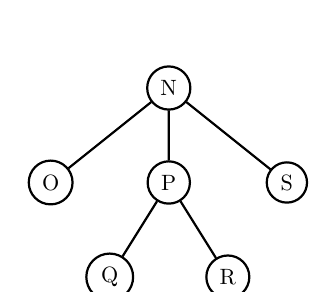
\begin{tikzpicture}
	[thick,scale=1, every node/.style={scale=0.8}]
	\node [circle,draw] {N}
	child {node [circle,draw] {O}}
	child {node [circle,draw] {P}
			child {node [circle,draw] {Q}}
			child {node [circle,draw] {R}}
		}
	child {node [circle,draw] {S}};
\end{tikzpicture}

queue\\
N\\
O P S\\
P S\\
S Q R\\
Q R\\
R

sequence: N O P S Q R

\newpage


\question{3}{(2+3pts) Recurrence Relations}
For each question, find the asymptotic order of growth of $T(n)$ i.e. find a function $g$ such that $T(n) = O(g(n))$. You may ignore any issue arising from whether a number is an integer. You can make use of the Master Theorem, Recursion Tree or other reasonable approaches to solve the following recurrence relations.

\textit{Note: \textbf{Mark or circle} your final answer clearly.\\ }

\begin{Q} $T(n) = 4T(n/2) + 42\sqrt{n}$.
\end{Q}

According to Master Theorem, $a=4,b=2,d=\frac{1}{2}$.\\
$\log_{b}a=\log_24=2>\frac{1}{2}=d$.\\
So, $\boxed{T(n)=O(n^2)}$

\vspace{6cm}
\begin{Q} $T(n) = T(\sqrt{n}) + 1$. You may assume that $T(2)=T(1)=1$.
\end{Q}

$T(1)=T(2)=1$\\
$T(4)=T(2)+1=2$\\
$T(16)=T(4)+1=3$\\
By induction, $T(2^{2^k})=k+1$\\
Let $n=2^{2^k}$, then we have $k=\log_2\log_2n$.\\
So, $\boxed{T(n)=O(\log{\log n})}$

\newpage
\question{3}{(7+6+6pts) Divide and Conquer Algorithm}

\begin{Q}
	In this problem, we will find an alternative approach to the merge step in Merge Sort named \textbf{Slice Merge} . Suppose $A$ and $B$ are sorted arrays with possibly different lengths, and let $n=len(A)+len(B)$. You may assume $n$ is a power of two and all $n$ elements have distinct value. The slice merge algorithm, \textbf{smerge(A,B)}, merges $A$ and $B$ into a single sorted arrays as follows:

	\begin{figure}[htbp]
		\centering
		\includegraphics[width=1.0\linewidth]{2}
	\end{figure}

	\textbf{Step 1:} Find index $s$ for subarray A and index $t$ for subarray B ($s+t=\dfrac{n}{2}$) to form two prefix subarrays \texttt{A[:s]} and \texttt{B[:t]}, such that \texttt{A[:s]} $\cup$ \texttt{B[:t]} contains the smallest $\dfrac{n}{2}$ elements in all $n$ elements of $A\cup B$.\\

	\textbf{Step 2:} Recur for \texttt{X = smerge(A[:s], B[:t])} and \texttt{Y = smerge(A[s:], B[t:])} respectively to reorder and merge them. Return their concatenation $X+Y$, a sorted array containing all elements in $A\cup B$.\\

	For example, if $A=[1, 3, 4, 6, 8]$ and $B=[2, 5, 7]$, we should find $s=3$ and $t=1$ and then recursively compute:

	\centerline{\texttt{smerge([1, 3, 4], [2]) + smerge([6, 8], [5, 7]) = [1, 2, 3, 4] + [5, 6, 7, 8]}}

	\vspace{0.5cm}
	\begin{enumerate}[1.]
		\item  Describe an algorithm for Step 1 to find indices $s$ and $t$ in $O(n)$ time using $O(1)$ additional space. Write down your main idea briefly (or pseudocode if you would like to) and analyse the runtime complexity of your algorithm below. You may assume array starts at index 1. \textbf{(2pts)}

		      \textbf{Algorithm Design}:
		      \begin{enumerate}
			      \item Set s and t equal to 0.
			      \item If $s+t$ is less than $n/2$, compare A[s] and B[t], let the smaller one's index plused by 1.
			      \item Repeat last step until once the condition is unsatisfied.
			      \item Then we get s and t.
		      \end{enumerate}

		      \textbf{Pseudocode}:
		      \begin{algorithm}[H]
			      \begin{algorithmic}[1]
				      \State s = t = 0
				      \While{s + t < n/2}
				      \If {A[s] < B[t]}
				      \State s++
				      \Else
				      \State t++
				      \EndIf
				      \EndWhile

			      \end{algorithmic}
		      \end{algorithm}
		      \textbf{Time Complexity Analysis}:\\
		      $T(n)=O(n/2)=O(n)$

		      \vspace{1.5cm}
		\item Write down a recurrence for the runtime complexity of \texttt{smerge(A,B)} when $A \cup B$ contains a total of $n$ items. Solve it using the Master Theorem and show your calculation below.\textbf{(2pts)}\\
		      Note: Write your answer for time complexity in asymptotic order form i.e. $T(n)=O(g(n))$.

		      $T(n)=2T(n/2)+O(n)$\\
		      According to Master Theorem, $a=2,b=2,d=1$,\\
		      $\log_ba=\log_22=1=d$,\\
		      so, $T(n)=O(n\log n)$
		      \vspace{1.5cm}
		\item Recall the merge step \texttt{merge(A,B)} to combine two subarrays of length $n/2$ in the Merge Sort algorithm covered in our lecture slides. Compare the runtime complexity of \texttt{smerge(A,B)} with \texttt{merge(A,B)}.\textbf{(1pts)}

		      The time complexity of smerge is $O(n\log n)$.\\
		      The time complexity of merge is $O(n)$.

		      \vspace{2.5cm}

		\item  Replace \texttt{merge(A,B)} by \texttt{smerge(A,B)} in the merge stage of Merge Sort to develop a new sorting method namely \textbf{S-Merge Sort}. Write down a recurrence for the runtime complexity of S-Merge Sort. Solve it and show your calculation below.\textbf{(2pts)}\\
		      Note: Write your answer for time complexity in asymptotic order form i.e. $T(n)=O(g(n))$.
		      \begin{align*}
			      T(n) & =2T(n/2)+O(n\log n)                        \\
			           & =2(2T(n/4)+O(n/2\log (n/2)))+O(n\log n)    \\
			           & =4T(n/4)+2O(n/2(\log n-\log 2))+O(n\log n) \\
			           & =4T(n/4)+2O(n\log n)-O(n\log 2)            \\
			           & =\dots                                     \\
			           & =\log n \times O(n\log n)                  \\
			           & =O(nlog^2n)
		      \end{align*}
	\end{enumerate}
\end{Q}
\newpage

\begin{Q}
	There are $n$ students in SIST and each student $i$ has $2$ scores $A_i$ and $P_i$, score in Algorithms and Data Structures course and score in Probabilty and Statistics course respectively. Students $i$, $j$ could form a mutual-help pair in CS101 class if and only
	if $A_i < A_j$ and $P_i > P_j$ . How many possible mutual-help pairs $(i,j)$ could be formed in CS101 class?

	Design an efficient algorithm  to figure out this problem. For comparison, our
	algorithm runs in $O(n \log n)$ time. (Hint: how to count inversions?)\\

	Note: Your answer should be consistent with the template we provide in Problem 0 Example.
\end{Q}

\textbf{Algorithm Design:}
\begin{enumerate}
	\item Make a Student Class which contains two properties, one is A (score in Algorithms and Data Structure course), the other is P (core in Probabilty and Statistics course).
	\item Use merge sort to sort all Students by their A in ascending order.
	\item Then, use merge sort to sort all Students again but by their P in ascending order, while finding how many inversions there are.
	\item Such as $A_i<A_j$ and $P_i>P_j$, so i goes before j after the first sort, but they should be found an inversion in the second sort, vise versa. Therefore, the number of inversions is the number of mutual-help pairs.
\end{enumerate}
\textbf{Pseudocode}:

A pair counter:
\begin{algorithm}[H]
	\begin{algorithmic}[1]
		\State count = 0;
	\end{algorithmic}
\end{algorithm}
A normal mergesort, ascending by A:
\begin{algorithm}[H]
	\begin{algorithmic}[1]
		\Function{mergesort1}{Student arr[], int head, int tail}
		\State mid = (head + tail) / 2;
		\State mergesort1(arr,head,mid);
		\State mergesort1(arr,mid,tail);
		\State i1 = i2 = k = 0;
		\While{i1 < n1 and i2 < n2}
		\If{arr1[i1].A < arr2[i2].A}
		\State arr[k] = arr1[i1];
		\State i1++;
		\Else
		\State arr[k] = arr1[i2];
		\State i2++;
		\EndIf
		\State k++;
		\EndWhile
		\EndFunction
	\end{algorithmic}
\end{algorithm}

A mergesort ascending by P, counting inversions:
\begin{algorithm}[H]
	\begin{algorithmic}[1]
		\Function{mergesort2}{Student arr[], int head, int tail}
		\State int mid = (head + tail) / 2;
		\State mergesort1(arr,head,mid);
		\State mergesort1(arr,mid,tail);
		\State i1 = i2 = k = 0;
		\While{i1 < n1 and i2 < n2}
		\If{arr1[i1].P < arr2[i2].P}
		\State arr[k] = arr1[i1];
		\State i1++;
		\Else
		\State arr[k] = arr1[i2];
		\State i2++;
		\State count++;
		\EndIf
		\State k++;
		\EndWhile
		\EndFunction
	\end{algorithmic}
\end{algorithm}

Function finding pairs:
\begin{algorithm}[H]
	\begin{algorithmic}[1]

		\Function{findPairs}{Student arr[],int n}
		\State mergesort1(arr,0,n);
		\State mergesort2(arr,0,n);
		\State return count;
		\EndFunction

	\end{algorithmic}
\end{algorithm}

\textbf{Complexity Analysis:}

Each mergesort in the function is $O(n\log n)$ .($T(n)=2T(n/2)+O(n),T(1)=\Theta(1)$, by Master Theorem, $T(n)=O(n\log n)$.)

Totally two mergesort in this function, so $T(n)=O(n\log n)+O(n\log n)=O(n\log n)$.




\newpage

\begin{Q}
	Suppose you are a teaching assistant for CS101, Fall 2077. The TA group has a collection of $n$ suspected code solutions from $n$ students for the programming assignment, suspecting them of academic plagiarism. It is easy to judge whether two code solutions are equivalent with the help of ``plagiarism detection machine'', which takes two code solutions \texttt{(A,B)} as input and outputs \texttt{isEquivalent(A, B)} $\in$ \{\texttt{True}, \texttt{False}\} i.e. whether they are equivalent to each other.

	TAs are curious about whether there exists a \textbf{majority} i.e. an \textbf{equivalent class of size $>\dfrac{n}{2}$} among all subsets of the code solution collection. That means, in such a subset containing more than $\dfrac{n}{2}$ code solutions, any two of them are equivalent to each other.

	Assume that the only operation you can do with these solutions is to pick two of them and plug them into the plagiarism detection machine. Please show TAs' problem can be sloved using $O(n\log n)$ invocations of the plagiarism detection machine.\\

	Note: Your answer should be consistent with the template we provide in Problem 0 Example.

	\noindent
\end{Q}

\textbf{Algorithm Design:}

\begin{enumerate}
	\item Make use of mergesort, divide the sequence into two equal pieces each turn, until the size of the subsequence is 1.
	\item For each subsequence, there can be a major value, and the number of times it occurs. Record both of them as \textbf{m} and \textbf{t}, respectively. If there is none, set $m = none$ and $t = 0$.
	\item When merging two sequences, following these rules:
	      \begin{enumerate}
		      \item If both sequences have their $m=none$ and $t=0$, we can simply set $m=none$ and $t=0$ for the merged sequence.
		      \item If one of the sequence have its $m=none$ and $t=0$, while the other does not, we can traverse the sequence whose $m=none$, counting how many numbers is equivalent to the other's $m$, add it to the other's $t$ to form a new pair of m and t for the merged sequence.
		      \item If both sequences have an equal m coincidentally (which is not none), just set the sum of two $t$ as a new $t$ for the merged sequence, and inherit the $m$.
		      \item If the two sequences have different m, saying m1 and m2 respectively, corresponding to t1 and t2, we would traverse both sequence and count how many opponent's m occurs in this sequence.(i.e. traverse sequence one to find how many times m2 occors, and add it to t2; traverse sequence two to find how many times m1 occors, and add it to t1). Then compare t1 with t2, set the t for the merged sequence as the lager one of them, and its corresponding m as the new m.(i.e. if t1>t2, t=t1, m=m1).
		      \item After all these steps, judge whether the t for the merged sequence is greater than n/2 (half size of the sequence). If it's true, we can keep the m and t, else, just reset it as $m=none,t=0$.
	      \end{enumerate}
\end{enumerate}

\textbf{Pseudocode}:

\begin{algorithm}[H]
	\begin{algorithmic}[1]
		\Function{findMajority}{Student arr[], int head, int tail}
		\If{head == tail}
		\State return;
		\EndIf
		\State mid = (head + tail) / 2;
		\State (m1,t1) = findMajority(arr[],head,mid);
		\State (m2,t2) = findMajority(arr[],mid,tail);
		\If{m1==none and m2==none}
		\State (m,t) = (none,0);
		\EndIf
		\If{m1==none and m2!=none}
		\State t1 += traverse sequence two to find how many m1
		\State (m,t) = (m1,t1);
		\EndIf
		\If{m1!=none and m2==none}
		\State t2 += traverse sequence one to find how many m2
		\State (m,t) = (m2,t2);
		\EndIf
		\If{m1!=none and m2!=none}
		\State t1 += traverse sequence two to find how many m1
		\State t2 += traverse sequence one to find how many m2
		\State t = max(t1,t2);
		\State m = corresponding to t
		\EndIf
		\If{t<=n/2}
		\State (m,t) = (none,0);
		\EndIf
		\State return (m,t);
		\EndFunction
	\end{algorithmic}
\end{algorithm}

\textbf{Complexity Analysis:}

The same as mergesort, we solve the problem by Divide and Conquer:

$T(n)=2T(n/2)+O(n)$, and $T(1)=\Theta(1)$,
according to Master Theorem, $a=2,b=2,d=1$, \\so $T(n)=O(n\log n)$.

\end{document}